\documentclass[usenatbib]{mnras}
\usepackage{siunitx}
\usepackage{graphicx}	% Including figure files
\usepackage[utf8]{inputenc}
\usepackage[english]{babel}
\usepackage{float}
\usepackage{amssymb, amsmath, yhmath}
\usepackage{verbatim}

\newcommand{\expect}[2]{\left< #1 \right| #2 \left| #1 \right>}
\renewcommand{\d}[1]{\! \mathrm{d}#1 \:}
\newcommand{\deriv}[2]{\frac{\d{#1}}{\d{#2}}}
\newcommand{\pderiv}[2]{\frac{\partial{#1}}{\partial{#2}}}
\newcommand{\parsq}[2]{\frac{\partial^2{#1}}{\partial{#2}^2}}


\bibliographystyle{mnras}
\setlength{\bibhang}{1in}
\setcitestyle{authoryear, open={(},close={)}}
\renewcommand{\bibsection}{\section*{References}}

\usepackage{graphicx}

\newcommand{\squote}[1]{\lq #1\rq}

\renewcommand{\d}[1]{\ensuremath{\operatorname{d}\!{#1}}}
\newcommand{\poweV}[1]{\SI{e#1}{\electronvolt}}
\newcommand{\ineV}[2]{\SI{#1 e #2}{\electronvolt}}
\newcommand{\lcdm}{$\Lambda$CDM}
\DeclareSIUnit\parsec{pc}
\DeclareSIUnit\lightyear{ly}
\DeclareSIUnit\year{yr}
\sisetup{range-phrase=--}
\sisetup{range-units=single}

\begin{document}

\title[Dark Matter Heating]{Heating of Milky Way disc Stars by Dark Matter Fluctuations in Cold Dark Matter and Fuzzy Dark Matter Paradigms}
\author[B. V. Church and J. P. Ostriker]{
Benjamin V. Church$^{1}$ \thanks{Contact e-mail: bvc2105@columbia.edu}, Philip Mocz$^{2}$ \thanks{Einstein Fellow},
Jeremiah P. Ostriker$^{1}$ \thanks{Contact e-mail: jpo@astro.columbia.edu}
\\
$^{1}$Columbia University, Department of Astronomy, New York, NY 10025, USA.
\\
$^{2}$Department of Astrophysical Sciences, Princeton University, 4 Ivy Lane, Princeton, NJ, 08544, USA.}
\maketitle
\begin{abstract}
Although highly successful on  cosmological scales, Cold Dark Matter (CDM) models predict unobserved over-dense \squote{cusps} in dwarf galaxies and overestimate their formation rate. We consider an ultra-light axion-like scalar boson which promises to reduce these observational discrepancies at galactic scales. The model, known as Fuzzy Dark Matter (FDM), avoids cusps, suppresses small-scale power, and delays galaxy formation via macroscopic quantum pressure. We compare the substructure of galactic dark matter halos comprised of ultra-light axions with masses $\poweV{-24} \leq m_a \leq \poweV{-18}$ to conventional CDM results. Besides self-gravitating subhalos, FDM includes additional substructure in the form of non-virialized over-dense wavelets formed by quantum interference patterns which provide a more efficient source of heating to galactic discs than do subhalos. We find that, in the solar neighborhood, wavelet heating is sufficient to give the oldest disc stars a velocity dispersion in excess of \SI{30}{\kilo\meter\per\second} within a Hubble time if all energy delivered to the disc goes into velocity dispersion. 
Furthermore, we calculate the radius-dependent disc velocity dispersion and corresponding scale height caused by the heating of dynamical substructure in both CDM and FDM with the determination that these effects will produce a flaring that terminates the Milky Way disc at \SIrange{15}{20}{\kilo \parsec}. Although the source of thickened discs is not known with any certainty, the heating due to perturbations caused by dark substructure cannot exceed the total disc velocity dispersion. Therefore, this work provides a lower bound on the FDM particle mass of $m_a > 0.57 \times \SI{e-22}{\electronvolt}$. FDM wavelets should be considered a viable mechanism for producing the observed disc thickening with time.
\end{abstract}

\begin{keywords}
cosmology: theory -- dark matter -- galaxies: structure
\end{keywords}

\section{Introduction}

The dark sector contributes a sizable majority of all matter in the universe. The existence of one or more kinds of dark matter is essential to galaxy formation and consistency with observed disc rotation curves. Over-dense regions of dark matter collapse to roughly localized concentrations of matter called ‘halos’ which are well-described by approximately spherically symmetric density profiles \citep{structure}. However, similar halos may vary significantly from these profiles in small-scale power i.e. substructure. Various models for the underlying physics of dark matter predict various patterns of density irregularities which, though invisible to the electromagnetic spectrum, are capable of perturbing the orbits of stars via gravitational effects. We will attempt to estimate those effects on the observable stars in galactic discs to better constrain our understanding of the fundamental nature of the dark matter.
             
\par 

The standard cosmological model (\lcdm) contains a massive electromagnetically non-interacting component known as Cold Dark Matter (CDM) with density parameter $\Omega_c = 0.259 \pm 0.006$ \citep{planck}. The properties of this substance are largely unknown and are assumed to be approximately that of a perfect fluid with negligible pressure compared to its energy density i.e. comprised of cold or non-relativistic matter at high redshift. CDM simulations suggest that substructure forms self-gravitating clumps which are qualitatively similar to free dark matter halos. We adopt a substructure formalism which tracks subhalos as an estimate of total substructure. The secondary gravitational effects of these subhalos is dependent on the subhalo mass function and the shape of small halo profiles, which is directly dependent on properties of the dark matter physics under consideration. Constraints obtained from The Sloan Digital Sky Survey measurement of Ly-$\alpha$ forest power spectra and surveys of dwarf galaxies below the free-streaming scale rule out most models of relativistic (hot) matter as the primary component of dark matter \citep{can_neutrinos}. Attempts to directly detect CDM particles in various plausible models of physics beyond the standard model have so far been without success \citep{direct_detection}.
	  
\par

Although amazingly accurate on cosmological scales, CDM models fail to make accurate predictions when compared with observations at distance scales less then \SI{1}{\kilo\parsec}. When compared with studies of dwarf galaxy rotation curves, CDM predicts unobserved density \squote{cusps} in the center of dark matter halos \citep{ultralight}. This failure is known as the \squote{cusp-core problem}. Another serious concern is the \squote{missing satellite problem}  \citep{missing_satellites}. The number of satellite galaxies predicted for a milky-way-like galaxy is greater than what we observe by an order of magnitude. This issue is sharpened by the \squote{too big to fail} problem of galaxy formation that claims some of the predicted satellites are so massive that it is difficult to imagine that they would not form any stars \citep{too_big_to_fail}. Various complex phenomena have been suggested as solutions to these problems such as baryonic feedback mechanisms which redistribute matter or  hypothetical dark matter self-interactions.

\par

An alternative model being studied known as Fuzzy Dark Matter (FDM) characterizes the bulk of dark matter as comprised of ultra-light($m \approx \poweV{-22}$) bosons whose characteristic de Broglie wavelength is on the order of $\SI{1}{\kilo\parsec}$. Such ultra-light particles are possible in various theories beyond the standard model \citep{axion_cosmology}. In particular, the class of axion-like particles is a perfect candidate for FDM and therefore, we refer to the mass of the constituent particles of FDM as the axion mass $m_a$. Macroscopic quantum mechanical wave effects “smear” the density profile on scales less than $\sim \SI{1}{\kilo\parsec}$ which removes problematic cusps from the center of large halos. These cusps are replaced by dense self-gravitating quantum states known as soliton cores which may facilitate indirect observational evidence for FDM. Furthermore, the quantum mechanical pressure caused by the large wavelength of FDM suppresses the formation of low-mass halos and entirely eliminates the formation of any halo or subhalo smaller than this wavelength, reducing or eliminating the missing satellites problem \citep{substructure_FDM}. Significant further effort remains in determining further discrepancies between FDM and CDM and whether these can, in conjunction with observational constraints, rule out one or both of the models.
 
\par

The dynamical effects of CDM have been studied in some detail, especially regarding the accretion and tidal stripping of CDM subhalos by large galaxies and their associated dark matter halos. On the other hand, research on the dynamics of FDM distributions is developing rapidly (c.f. \cite{schive_solitons, Schrodinger-Poisson, Schive-virialized-wave-halos}) but still is in its infancy. However, dynamical studies have focused on simulations which inherently have a fixed resolution and thus are limited to small (approximately \SI{1}{\mega \parsec} scales) cosmological volumes and low ($M << 10^{12} M_{\odot}$) halo masses. In this paper, we present analytic estimates for substructure dynamical fluctuations which do not suffer from limited resolution. The resolution limit of simulations causes underestimates of subhalo populations and therefore to their dynamical effects. 
\par 
	CDM and FDM models predict significant differences in the distribution of halo substructure. While CDM predicts a power law divergence in the number of small subhalos, the FDM subhalo mass function approaches zero below a cutoff scale determined by the axion mass expressed by the Jean’s scale at which quantum pressure and gravitational attraction balance:
\setlength{\belowdisplayskip}{4pt} \setlength{\belowdisplayshortskip}{4pt}
\setlength{\abovedisplayskip}{4pt} \setlength{\abovedisplayshortskip}{4pt}

\begin{equation}
k_J = 66.5 \cdot (1+z)^{1/4} \left( \frac{\Omega_a h^2}{0.12} \right) \left(\frac{m_a}{\poweV{-22}} \right)^{1/2} \si{\per\mega\parsec},
\end{equation}
\noindent
as given by \citet{axion_cosmology}. \\ For ultra-light axions, the subhalo mass function is significantly suppressed though the entire range of substructure for a halo comparable to the Milky Way’s. However, FDM subhalos will exhibit solitons which, for moderately-sized subhalos and large axion masses, are very dense and largely unaffected by tidal disruption. The main deviation from CDM phenomena occurs on scales smaller than the coherence length. Above this scale, the Schr\"{o}dinger-Poisson–Vlasov-Poisson correspondence predicts that the self-gravitating nonlinear Schr\"{o}dinger equation governing FDM reproduces the physics of collisionless particulate dark matter \citep{Schrodinger-Poisson}. Simulations using zoom-in techniques are able to resolve complex structure in the core of an FDM halo and have discovered large-amplitude oscillations in the core density of such halos \citep{structure-FDM-halos}. In addition, a surprising standing wave phenomenon has been observed in the density profiles produced by small-scale FDM computer simulations \citep{cold_and_fuzzy}. These standing waves, named wavelets, radically alter the dark matter profile and may, through gravitational interactions, disturb the baryonic components in directly measurable ways. The primary effect of these wavelets is to introduce time-varying perturbations to the gravitational potential on a much shorter time-scale than the evolution of primary structure after the system has come into virial equilibrium \citep{Schrodinger-Poisson}. 
\par
	The velocity dispersion of stars in a galactic disc provides a proxy to study the gravitational perturbations produced by the dark matter halo substructure. We know that the dispersion increases with age via an approximate power law $\sigma \propto t^\beta$ \citep{heating_history}. Therefore, the best observational bounds on the amount of gravitational substructure will come from the analysis of old, thick disc stars.  

\section{Galactic discs}

\hspace{5mm} Current observations suggest that the discs of spiral galaxies may be roughly modeled by an approximately exponential profile in radius and in vertical structure. The vertical scaling is determined by the mass density of the disc and the perpendicular velocity dispersion.  The bulk of the stars in normal discs are divided into a cold `thin disc' of relatively young stars and a hot `thick disc' of old stars \citep{binney_tremaine_2008}. 

The identification of and first evidence for the presence of a thick disc in the Milky Way Galaxy was presented by \cite{milkyway-thickdisc} who showed that the  density profile of stars as a function of distance from the galactic plane could not be explained by a single exponential, but rather by two exponentials with scale heights of $\SI{300}{\parsec}$ and $\SI{1350}{\parsec}$ respectively.
The vertical velocity dispersion and therefore scale height of the old stars is significantly greater which is why this population is referred to as the `thick disc'. Stars in the thick disc are very old, most with ages exceeding \SI{12}{\giga \year} and the majority of thick disc sub-giants dating from 12 - \SI{13}{\giga \year} ago \cite{age_of_thick_disc}. In comparison, the stars comprising the thin disc have a much wider range of ages, most younger than $\SI{8}{\giga \year}$. 
Subsequent studies have established chemical differences in metallicity and $\alpha$-abundance between the stars in the thin and thick discs with the thin disc consisting of the younger high metallicity population I stars \citep{GALAH_thick_disc, chemical_thick_disc}. Although the thick disc is the older of the two, it ought not be confused with the \textit{old} disc which refers to the older component stars of the \textit{thin} disc. Such terminology is used because the thin disc is comprised of stars with a broad range of ages.  
\par
Studies of the velocity dispersion of Milky Way stars at varying angles and scale heights showed that the velocity dispersion of the thick disc is time dependent and fit approximately by a power law $\sigma_D \propto t^{\beta}$ where the best estimates for the exponent are $\beta \approx 0.3$ \citep{heating_history}. The origin of this disc structure is unknown but there are three widely considered explanations. One hypothesis is that the thick disc formed with subsequent stellar generations born in ever slimmer discs due to energy loss of the disc to gas shocks. However, this explanation struggles to explain the profile of observed decrease in velocity dispersion with increasing redshift \citep{emergence-thick-disc}. An alternative hypothesis is that tidal interactions between galaxy close encounters can inject energy into existing stars which effectively puffs up the disc \citep{thick-disc-mergers}. \cite{mergers} ruled our major mergers in the accretion history of the Milky Way which are inconsistent with the existence of a cold disc and further limit the total mass of stars or dark matter which could have been accreted to at most 4\% of the mass of the galaxy (interior to $R_{\odot}$) over the lifetime of the Milky Way. Furthermore, estimates of the actual rate of accretion onto spiral galaxies are consistent with this limit and large enough for the accretion of dwarf satellites to be a viable mechanism explaining observed disc thickness \citep{mergers}.
The recent study by \cite{gaia_normal_process} based on Gaia data revives the proposal that the thick disc was produced by the ancient accretion of an Small Magellanic Cloud-like satellite system. This otherwise attractive possibility would not produce the age-velocity dispersion observed in the Milky Way thick disc. 
A final possibility, and the mechanism we consider in this paper, is that the thick disc is formed by continually heating older stars \citep{thin-and-thick-disc}. 
\par 
Assuming that galactic disc components are formed by continual heating, the primary source of this heating remains uncertain. Interactions between spiral modes and radial migration of stars due to spiral arms have been proposed as a mechanism for heating spiral discs \citep{radial_migration}. However, the ability to heat up to the velocity dispersion of the old disc stars by spiral modes remains to be demonstrated. The time-varying quadrupole moment of the bar of a barred spiral galaxy can also drive vertical disc heating. \cite{vertical_heating_modes} show that, in cosmological-zoom calculations of Milky Way like CDM halos, rotating bars are the dominant effect while spiral density waves and radial migration are sub-dominant. Furthermore, they find that dynamical subhalos and satellites with masses above $10^{10} M_{\odot}$ dominate all the above disc-disc interactions. 
Although spiral arms couple weakly to the vertical motions of stars, such effects are able to efficiently increase their planar velocity distribution which, in turn, are converted into vertical motions by giant molecular clouds (GMCs) acting as scattering centers \citep{vertical_structure_and_GMC}. Combined GMC and spiral/bar heating is successful in explaining the age-velocity dispersion relation for the galactic thin disc but is unable to produce the thick disc of a Milky Way like galaxy \citep{heating_history}.
Here we will consider the possibility that disc heating is caused by interactions with dynamical dark halo substructure, for instance, subhalos. In this case, we will be able to sharply restrict the parameter space of possible dark matter paradigms. Regardless of the origin of thick discs, the heating due to dark substructure can at most account for the total observed velocity dispersion of the thick disc. Therefore, these results are able to put a lower bound on the mass of the FDM axion which is agnostic to the mechanism behind producing thick discs.
\par
The discs of normal spiral galaxies approximately follow an exponential radial density profile,
\begin{equation}
\rho(r, z) = \frac{\Sigma_0}{2 h(r)} e^{-r/r_0} \mathrm{sech}^2{(z/h(r))}, 
\end{equation}
where $r_0$ is the scaling radius and $h(r)$ is the scale height at a given radius. The indicated vertical dependence is exact only for a disc which is isothermal along vertical slices of constant radius. Furthermore, the projection of the mass density onto the galactic plane has the same exponential form. In particular, the local surface density as a function of radius has approximately the form,
\begin{equation}
\Sigma(r) = \int_{-\infty}^{\infty} \rho(r, z) \d{z} = \Sigma_0 e^{-r / r_0}.
\end{equation}
For the Milky Way the local surface density is estimated to be $\Sigma_{\odot} = \SI{68}{M_{\odot} \per \parsec \squared}$ using dynamical measurements \citep{dynamical_measurement}. We take the Milky Way disc to have an exponential surface density profile with $r_0 \approxeq 3.2$ to fit the estimated component-wise rotation curve of \cite{milky_way_halo}. The vertical profile is determined by hydro-static equilibrium under the gravity from the planar density distribution of the disc with pressure supporting the vertical structure is given by the vertical velocity dispersion $P = \rho \sigma_D^2$,
\begin{equation}
- 4 \pi G \rho = \frac{\partial^2 \phi}{\partial z^2} = \pderiv{}{z} \left( \frac{1}{\rho} \pderiv{ \rho \sigma_D^2}{z} \right).
\end{equation}  
Therefore, integrating through the disc and approximating $\sigma_D^2$ as varying slowly vertically through the disc we arrive at the following expression relating the scale height and vertical velocity dispersion of the disc:
\begin{equation} \label{scale}
4 \pi G \Sigma(r) = \frac{ \sigma_D(r)^2 }{h(r)}.
\end{equation}
Stars oscillating vertically through the disk are acted on by a gravitational acceleration and corresponding gravitational potential,
\begin{subequations}
\begin{align}
-\mathbf{g}(z) & = 4 \pi G \int_0^z \rho(r, z') \d{z'} = 2 \pi G \Sigma \: I_1(z / h) ;
\\
I_1(y) & = \int_0^y \sinh^2(x) \d{x} .
\\
\phi(z) & = - \int_0^z \mathbf{g}(z') \d{z'} = 2 \pi G \Sigma \: h \: I_2(z / h) ; 
\\
I_2(y) & = \int_0^y I_1(x) \d{x}.
\end{align}
\end{subequations}
Thus, the vertical oscillations of such a star with maximum vertical height $z_m$ have a period given by,
\begin{subequations}
\begin{align}
\frac{P}{2} & = \int_{-z_m}^{z_m} \frac{\d{z'}}{\sqrt{2(\phi(z_m) - \phi(z'))}} = \sqrt{\frac{h}{4 \pi G \Sigma}} J(z / h) ;
\\
J(y) &= \int_{-y}^y \frac{\d{x}}{\sqrt{I_2(y) - I_2(x)}} .
\end{align}
\end{subequations}
The function $J$ is monotonically increasing and bounded below by $\pi \sqrt{2}$. 
Using the disc scale height to velocity dispersion relation given by equation \eqref{scale}, the vertical oscillation period can be written as,
\begin{equation} \label{period}
P = \frac{2 \sigma_D}{4 \pi G \Sigma} J(z_m / h) = \frac{2 h}{\sigma_D} J(z_m / h)
\end{equation}
The period of disc oscillations determines the adiabatic cutoff for heating due to perturbing interactions. The velocity dispersion of the disk, $\sigma_D$, corresponds to the thin disk and the gas fueling star formation. We assume that disk stars are born with the velocity dispersion of the gas and their velocity profile evolves from there due to heating. The extremities of the thick disk is formed from stars which evolved from the small proportion of stars with large $z_m$ on the order of $2$ to $3$ scale heights. Under the assumption that disc thickening is due primarily to the proposed dark substructure dynamics, the dependence on radius of the disc velocity dispersion $\sigma_D$ can be calculated explicitly. Using the above relations and the radial dependence of $\sigma_D$ we can predict the radial thickness profile of the galactic disc and compare these results to measurements of the flaring of actual discs.  
\par
We now turn our attention to the Milky Way which has the best studied galactic disc. \cite{milky_way} has performed a comprehensive study of the various distribution functions of Milky Way stars and, in particular, has compiled data on the velocity dispersion of the thin and thick discs as a function of vertical distance. \cite{milky_way} proposes a ``pseudo-isothermal'' distribution function for the velocity dispersion which has the form,
\begin{equation}
f_z(J_z) = \frac{\left( \Omega_z J_z + V_\gamma^2 \right)^{-\gamma}}{2 \pi \int_{0}^{\infty} \d{J_z} \: \left( \Omega_z J_z + V_\gamma^2 \right)^{-\gamma} },
\end{equation}  
in term of the action variable $J_z$. For stars in the solar neighborhood with $r \approx R_{\odot} =  \SI{8.3}{\kilo \parsec}$ the best fit parameters of $\gamma = 2.6$ and $V_\gamma = \SI{18.7}{\kilo \meter \per \second}$ give excellent agreement with survey data collected by \cite{milkyway-thickdisc}. Using this formalism, the main component of the perpendicular velocity dispersion of the thick disc is $\sigma_D = 32 \pm 1 \si{\kilo \meter \per \second}$ at the neighborhood near the solar radius $R_{\odot}$.   



\section{Heating via Substructure Dynamics}

We provide models for how dynamical halo substructure can heat galactic discs due to time-varying gravitational interactions. First we will consider self-gravitating substructure in both CDM and FDM of which the dominant form is approximately self-similar subhalos. Additionally, we will consider the peculiar feature of wave dark matter which produces time-dependent substructure on the order of the de Broglie wavelength due to interference. This wavelet substructure provides an additional source of heating which is qualitatively very different from the heating due to subhalos because the wavelets are not self-gravitating objects. 

\subsection{Estimating The Heating Due to Transits}

We first provide a rough analysis of the heating due to transiting over-dense regions of dark matter. Each transit causes a change in velocity of approximately,
\begin{equation}
\Delta v^2 = \left( \frac{M_l G}{b v_l} \right)^2,
\end{equation}
where $M_l$ is the mass of the region, $v_l$ is its velocity, and $b$ is the distance at closest approach. However, the heating is ineffective if these perturbations are adiabatic (i.e. slow compared to the oscillation period of the star in question) which will merely cause gradual periodic changes rather than overall heating to the orbits whose adiabatic invariants remain fixed. However, if the heating is roughly impulsive then the orbits will be irreversibly perturbed. The non-adiabatic condition approximately corresponds to the constraint,
\begin{equation} \label{adiabatic}
\frac{b}{v_l} < \frac{P}{2},
\end{equation}
where $P$ is the characteristic vertical period of the objects subjected to perturbation, in this case the period for lateral oscillations through the galactic disc. The heating of the disc is measured by tracking the one-dimensional velocity dispersion of the disc $\sigma_D^2 = \left< \dot{z}^2 \right>$ over time. The total rate of heating is therefore given by the accumulation of all such encounters,
\begin{subequations}
\begin{align}
\deriv{\sigma_D^2}{t} &= \int_{b_{\min}}^{b_{\min}} (2 \pi b) \: \d{b} \: n v_p \: \left( \frac{M_l G}{b v_p} \right)^2 ;
\\
& = \frac{M_l^2 G^2}{v_l} \: 2 \pi n \log{\Lambda},
\end{align}
\end{subequations}
where we have defined,
\begin{equation}
\log{\Lambda} \equiv \log{\left( \frac{b_{\text{max}}}{b_{\text{min}}} \right)},
\end{equation}
which is the gravitational equivalent of the Coulomb logarithm. Here $v_l$ is the relative velocity between the disc and the perturbing objects in the halo. 
The maximum distance across which the heating is efficient, $b_{\max}$, is fixed by equations \eqref{adiabatic} and \eqref{period} and the minimum distance, $b_{\min}$, is given by the characteristic size for the perturbing objects denoted, $r_{l}$. 
Therefore, in terms of the overall one-dimensional velocity dispersion, we derive the time-dependent heating as,
\begin{subequations}
\begin{align}
\deriv{\sigma_D^2}{t} &= \frac{M_l^2 G^2}{\sigma_H} \: 2 \pi n \log{\Lambda} ;
\\
\Lambda & = \frac{\sigma_H \sigma_D}{4 \pi G \Sigma \: r_l} J(z_m / h).
\end{align}
\end{subequations}
A more detailed calculation found in \cite{milkywayblackholes} gives somewhat altered numerical factors,
\begin{align} \label{heating}
\deriv{\sigma_D^2}{t} = \frac{8 \pi M_l^2 G^2}{\sqrt{2} \sigma_H} \: n \: \log{\Lambda}.
\end{align}
We define the quantities,
\begin{subequations}
\begin{align}
\sigma_{10} &= \left((\SI{10}{\giga \year}) \cdot \deriv{\sigma_D^2}{t} \right)^{1/2}  
\\
\sigma_{T} &= \left( \int_0^{\SI{10}{\giga \year}} \deriv{\sigma_D^2}{t} \;\; \d{t} + \sigma_{D,0}^2 \right)^{1/2}  
\end{align}
\end{subequations} 
as a standard measures of the approximate heating over an estimate of the age of a Milky Way-like halo.
\par
	An alternative approach for calculating heating due to transits is given by \cite{ultralight} which only considers the tidal effects on disc heating. That model assumes that only local dispersion acting across a characteristic scale much smaller than $H$ can lead to overall heating. However if processes such as outgoing density waves are an inefficient means for dissipating differential motions of the disc then dynamical friction between oscillating disc components will tend to dissipate oscillation energy into disc heating and therefore contribute to the thickening. In this analysis, we will assume that such processes are inefficient and therefore equation \eqref{heating} gives a reasonable estimate of the total rate of disc heating.  
\par	
	The calculation we provide is based on the total kinetic energy delivered into vertical motions of the disc. These motions can be broken in to two components: those reflecting a direct increase in the z-velocity dispersion and those invested in bending waves which give one part of the disc a z-velocity with respect to the mean disc velocity. Some fraction of the second component could be damped by transfer of energy back to the dark matter, to gas motions, or be transferred radially outwards in propagating bending disc waves. Thus, our calculation provides an upper bound on the disc heating by subhalos and wavelets with the calculation given by equation (37) of \cite{ultralight} giving a lower bound.   	

\subsection{Heating Due to Subhalos}

\subsubsection{Spatial Profile}

We model substructure as comprised entirely of subhalos which act as distinct massive particles subject only to gravitational attraction and tidal disruption. Following \citet{tidal_limit} and \cite{unified_model} we adopt a
simplified model of subhalo
formation and dynamics. The initial shape of
the subhalo mass function is assumed to
be spatially invariant, i.e. the position
and mass variables are decoupled. The
total density of subhalos is assumed to initially
follow the Navarro--Frenk--White (NFW) profile:
\begin{equation}
\rho(r) = \frac{\rho_0}{r/r_c (1+r/r_c)^2},
\end{equation} which also
describes the density profile of the
primary dark matter halo given by \citet{structure} from CDM simulations. This profile is fairly universal for the halos of massive cold particles which we assume accurately describe subhalos. Furthermore, we are working under the assumption that the primary modifications of subhalos relative to free halos arise from tidal stripping. Wave dark matter models modify the primary halo density profile away from NFW. The core behavior in FDM is primarily due to quantum pressure which does not act between self-gravitating lumps. Therefore, we do not expect the spatial distribution of subhalo formation to be significantly altered from FDM. That said, due to extreme tidal disruption, subhalos near the core of the primary halo contribute negligibly, so the exact shape of their distribution near the core is unimportant.  

\subsubsection{The Subhalo Mass Function}

The only additional information needed to calculate the perturbations due to subhalos is the distribution of subhalo populations as a function of mass. However, the tidal interactions between the primary halo and its interior subhalos complicates the elegant halo mass functions determined by the over-density correlation function and power spectrum. We approximate the subhalo populations by assuming that the unresolved subhalo mass function has the same form as the free halo mass function derived from the extended Press--Schechter formalism. The unresolved mass function is then modified by tidally truncating unresolved halos such that the unresolved halo mass function is shifted towards lower mass and the modified subhalo mass function becomes coupled in subhalo mass and radius inside the primary halo. Therefore, the population of subhalos is entirely determined by two functions, $\frac{\d{n}}{\d{\log{M}}}$, the unresolved (free) halo mass function, and $T_R(M)$, the truncated mass function at a radius $R$. 


\subsubsection{Calculating the Heating}

In terms of these functions, the rate of heating is given by,
\begin{equation} \label{subhaloheating}
\deriv{\sigma_D^2}{t} = \frac{8 \pi G^2}{\sqrt{2} \: \sigma_H} \int_0^{M} T_R(m)^2  \deriv{n}{m}  \log{\left( \frac{\sigma_H \sigma_D}{4 \pi G \Sigma \: r_{\text{t}}(m)} \right)} \d{m},
\end{equation}   
where $r_{\text{t}}(m)$ is the radius of a subhalo of mass $m$ after truncation at a radius $R$. 
If we assume that the primary halo and substructure formed quickly on the scale the lifetime of the disc, and that dark substructure dynamics in the form of transiting subhalos alone constitutes the primary source of disc thickening then equation \eqref{subhaloheating} gives the time-dependence of $\sigma_D$ as a function of time over the entire history of the halo. Furthermore, the rate of heating given by equation \eqref{subhaloheating} depends on $\sigma_D$ only logarithmically. Therefore, the square of the velocity dispersion increases at an approximately constant rate analogous to a random walk. Therefore, this heating model predicts an exponent, $\beta \approx \tfrac{1}{2}$ in the time dependence $\sigma_D \propto t^{\beta}$.

\subsection{Heating Due to Quantum Wavelets in FDM}

In models of wave dark matter, there is an added contribution to the fluctuating substructure due to interference of excited modes which produce time-dependent over-densities known as wavelets. Using results of the distribution of these wavelets given by numerical FDM simulations given by \cite{BECDM}, here we analytically estimate their dynamical heating impact. We assume that the density of the wavelets is a fixed multiple of the local mean density such that,
\begin{equation} \label{multiple_of_background}
M_w = A \left(\frac{\lambda_{\text{char}}}{2} \right)^3 \rho(r),
\end{equation}  
where $\lambda_{\text{char}}$ is the local characteristic scale of the wavelets. Because these wavelets are inherently produced by quantum mechanical interference, they will approximately saturate the uncertainty relations,
\begin{equation}
\lambda_{\text{char}} m_a \sigma_H \approx \hbar,
\end{equation}
where $m_a$ is the mass of the FDM particle or axion. However, the numerical factors in this relationship are important for giving an accurate bound on the particle mass. Therefore, we will provide a more detailed treatment. 
\par
The wavefunction encoding these wavelets can be constructed as follows. We assume that entire mass of the primary FDM halo (external to the central soliton) is in the form of wavelets such that,
\begin{equation} \label{const}
M_w n = \rho(r).
\end{equation}
Such is the case in simulations of idealized virialized FDM halos \citep{numerical-Schrodinger} These wavelets are a result of linear interference patters of the underlying velocity dispersion of particles $\sigma_H$. Classically, the particles would have an approximately Maxwell-Boltzmann distribution:
\begin{equation}
f(\mathbf{v}) \propto \exp\left(-v^2/(2\sigma_{H}^2/3)\right).
\end{equation}
Quantum mechanically, by the Schr\"{o}dinger-Poisson–Vlasov-Poisson correspondence, the wave function is given by:
\begin{equation} \label{phase_dist}
\psi(\mathbf{x}) \propto \sum_{\mathbf{v}} f(\mathbf{x},\mathbf{v})^{\frac{1}{2}} \exp{\left[i m \mathbf{x}\cdot\mathbf{v}/\hbar + 2\pi i \phi_{{\rm rand},\mathbf{v}} \right]}
\, \mathrm{d}^{3}{\mathbf{v}},
\end{equation}
(equation 27, \cite{Schrodinger-Poisson}) where $\phi_{{\rm rand},\mathbf{v}}\in[0,2\pi)$ is a random phase associated with velocity $\mathbf{v}$.
Such a constructed wavefunction is in agreement with local patches of the wavefunction seen in simulated idealized virialized halos \citep{BECDM}.
In such a distribution, structure is totally suppressed below the de-Broglie wavelength $\lambda_{\rm dB} \equiv \hbar/(m_a \sigma_H)$ by the uncertainty principle.
The characteristic size of these wavelets (determined numerically from the peak of the density power spectrum) is a multiple of the suppression scale:
\begin{equation} \label{characteristic_wavelength}
\lambda_{\text{char}} = \frac{ 2 \pi \hbar}{m_a \sigma_H \sqrt{\frac{3}{2}}}.
\end{equation}
The value of A in equation \eqref{multiple_of_background} can be then determined numerically for the distribution given by equation \eqref{phase_dist} as follows. First, a density field $\rho = |\psi|^2$ in a statistically large-enough box ($> 100$ de Broglie Wavelengths) is constructed according to equation \eqref{phase_dist} with velocity dispersion $\sigma_H$ and average density $\rho = \bar{\rho}$. The number of resulting density peaks per unit volume then gives $n$, which by the constraint of equation \eqref{const}, determines the average mass $M_w$ of the wavelets. Then, $A$ is deduced from equation \eqref{multiple_of_background} using equation \eqref{characteristic_wavelength} for the characteristic size. Numerically, we find $A\simeq 2.2$ for a wavefunction that encodes an underlying Maxwell-Boltzmann distribution.
\par
The heating due to wavelets is approximately given by,
\begin{subequations} \label{FDMheating}
\begin{align}
\deriv{\sigma_D^2}{t} & = \frac{2 \pi A}{3 \sqrt{3}} \left( \frac{2 \pi \hbar }{m_a} \right)^3 \frac{(\rho(r) G)^2}{\sigma_H^4} \log{\Lambda} ;
\\
\Lambda & = \frac{P \sigma_H}{\lambda_{\text{char}}} = \frac{m_a \sigma_H^2 \sigma_D}{4 \pi^2 \hbar G \Sigma} \sqrt{\tfrac{3}{2}} J(z_m / h) .
\end{align}
\end{subequations}
Therefore, using $\Sigma = \Sigma_0 e^{-r/r_0}$ we can express the rate of heating as a function of radius. Under the same assumptions that the considered dynamics are the dominant contribution to disc thickening, as before, the rate of heating given by equation \eqref{subhaloheating} depends on $\sigma_D$ only logarithmically. Therefore, the square of the velocity dispersion increases with an approximately constant rate analogously to a random walk. This heating model also predicts an exponent, $\beta \approx \tfrac{1}{2}$ in the time dependence $\sigma_D \propto t^{\beta}$. Once again we note that, since we are considering both components of disc heating as ultimately being reflected in the z-velocity dispersion, we here provide an upper bound on the effect. 
\par
We note that \eqref{FDMheating} is consistent with the general scaling symmetry of the Schr\"{o}dinger - Poisson equations which govern the dynamics of a self-gravitating quantum superfluid such as FDM:
\begin{equation}
\{ x, t , \rho, m \} \to \{\alpha x, \beta t, \beta^{-1} \rho, \alpha^{-2} \beta m \} .
\end{equation}
\noindent \citep{Schrodinger-Poisson}.
\subsection{Heating in the CDM Paradigm}

\subsubsection{Unresolved Mass Function}

As the primary halo forms, it captures subhalos via accretion. The unresolved subhalo mass function refers to the distribution of subhalo masses at the time of accretion before dynamical effects such as tidal stripping have biased the distribution. We assume the unresolved subhalo mass function is very close in shape to the free halo mass function truncated above the primary halo mass. Based on population statistics of subhalos in high resolution N-body simulations given by \citet{subhalo_abundance} we take this fraction to be $\sim 10\%$. The CDM halo mass function and corresponding subhalo mass function calculated from simulations \citep{pop_of_subhalos, unified_model} are well fit by a power law in the accretion mass $m_{acc}$ which denotes the mass of a subhalo before modification by the external tidal field. This form matches the free halo mass function, 
\begin{equation}
\frac{\d{n}}{\d{\: \log{m_{acc}}}} = C \left(\frac{\rho(r)}{M}\right) \left(\frac{m_{acc}}{M} \right)^{-p} ,
\end{equation}
with $p = 0.9$ and where $M$ is the mass of the primary or host halo.
Furthermore, we fix the total mass in (accreted) halos as a fraction of the total mass of the primary halo. Therefore,
\begin{subequations}
\begin{align}
M_{\mathrm{halos}} & = \int m \deriv{n}{(\log{m})} \d{(\log{m})} \d{V} ;
\\
& = C \int \left(\frac{\rho(r)}{M}\right) \left(\frac{m}{M} \right)^{-p} \d{m} \d{V} ;
\\
& = \frac{C}{1-p} \left[ \frac{(f_2 M)^{1-p}}{M^{-p}} \right] = f_1 M ,
\end{align} 
\end{subequations}
so we fix the constant,
\begin{equation}
C = (1 - p)\frac{f_1}{f_2^{1-p}} .
\end{equation}

\subsubsection{Tidal Disruption} 

We adopt a simplistic model of tidal stripping which underestimates the total effect. A tidal radius is calculated by setting the tidal force on a test mass equal to the gravitational attraction of the subhalo. The resulting radius is:
\begin{equation}
R_t = R \left(\frac{m_{\text{acc}}}{2 M(R)}\right)^{1/3} =  R_{\text{max}} \left(\frac{m_{\text{acc}}}{M}\right)^{1/3} f_T(R), 
\end{equation} 
with $f_T(R) \propto R/R_c(\log(1+R/R_c) - R/(R+R_c))^{-1/3}$, where $R_c$ is the core radius of the primary halo. This formula simply comes from the functional form of the enclosed mass as a function of radius for an NFW profile. We then suppose that total truncation occurs outside this radius and no disruption occurs within it. Thus,
\begin{equation}
\frac{T_R(m_{\text{acc}}}{m_{\text{acc}}} = 
\begin{cases}
\frac{\log{(1+R_t/r_c)} - R_t/(r_c+R_t)}{\log{(1+c)} - c/(1+c)},
& \text{if } R_t < r_{\text{max}}
\\
    1,              & \text{otherwise}
\end{cases}
\end{equation} 
However, $m_{acc} = 200 \rho_0 \frac{4}{3} \pi c(m)^3 r_c^3$ and $r_{\text{max}} = c(m) \: r_{c}$ so we get,
\begin{equation}
R_t = r_{\text{max}} f_T(R).
\end{equation}
Therefore,
\begin{equation} \label{trunc}
\frac{T_R(m_{\text{acc}})}{m_{\text{acc}}} =
\begin{cases}
\frac{\log{(1 + x)} - x/(1 + x)}{\log{(1+c)} - c/(1+c)},& \text{if } f_T(R) < 1
\\
1, & \text{otherwise}
\end{cases}
\end{equation} 
where $x = c(m) \cdot f_T(R)$. Since $c$ is a weak function of $m$, the remaining mass fraction is also a weak function of $m$. Therefore, in agreement with the results of \citet{unified_model}, the final resolved subhalo mass function is approximately also decoupled in mass and radius. High-resolution CDM simulations prominently exhibit the depletion of subhalos with orbits passing below $r < \SI{20}{\kilo \parsec}$ inside a halo like the Milky Way's. The cosmological high-resolution `zoom-in' simulations of a $M = 10^{12} M_{\odot}$ primary halo performed by \cite{subhalo_truncation_sims} show extreme depletion due to tidal effects of nearly all subhalos within $\SI{15}{\kilo\parsec}$. However, recent analytical estimates suggest that extreme depletion of subhalos due to total tidal disruption in state-of-the-art N-body simulations is, in fact, a numerical artifact \citep{dark_matter_substructure_numerics}. Furthermore, \cite{disruption_numerics} show that the dominant tidal influence on CDM subhalos is due to the tidal field of the host halo and disc rather than subhalo-subhalo interactions and that physical disruption of CDM substructure due to tidal stripping or shocks is extremely rare. Accordingly, the model we employ produces comparably gentler subhalo mass depletion in the range $10 - \SI{15}{\kilo \parsec}$ and heavily strips mass from all subhalos within $\SI{10}{\kilo\parsec}$ rather than completely disrupting them. \cite{subhalo_truncation_sims} conclude that the tidal field of the central galaxy is responsible for the severity of subhalo depletion and that the disc potential will primarily outright destroy transiting subhalos rather than partially strip their mass. Our underestimate of tidal disruption is due to neglecting to accurately account for the sharp tidal field of the galactic disc. However, we find that, within the range where the disc accounts for significant subhalo depletion, heating due to subhalo dynamics is unimportant. Therefore, we do not expect the detailed mechanism of tidal depletion to significantly affect our results. 

\subsubsection{Calculating the disc Heating}

For a Milky Way-like halo with $M = 0.8 \times 10^{12} \, M_\odot$ and $c = 15$ \citep{milky_way_halo}, we can calculate heating due to subhalos as a function of radius. We find that the rate of heating is quite weak in the core of the halo where tidal disruption is the dominant effect. However, as seen in figure \ref{fig:CDMheating}, subhalo heating becomes quite efficient near the solar neighborhood $R_{\odot} = \SI{8.3}{\kilo \parsec}$. In fact, at $R_{\odot}$ the rate of heating is $\frac{\d{\sigma_H^2}}{\d{t}} = \SI{0.19}{\kilo \meter \squared \per \second \squared \per \giga \year}$ which does accumulate over the lifetime of the galaxy to about 5\% of the observed velocity dispersion of $\SI{32}{\kilo \meter \per \second}$ at $R_{\odot}$. However, somewhat beyond the solar neighborhood at $r = \SI{17}{\kilo \parsec}$ the rate of heating jumps up to $\frac{\d{\sigma_H^2}}{\d{t}} = \SI{121.2}{\kilo \meter \squared \per \second \squared \per \giga \year}$ which is marginally in excess of the maximum rate allowed by the total velocity dispersion of the thick disc. However, it is difficult to obtain accurate distribution functions in the outer disc to compare this value to the actual velocity distribution of the thick disc. As the radius increases, heating due to subhalos becomes far more significant leading to a rapid flaring of the Milky Way disc and, eventually, destruction of the outer disc. Subhalo induced heating may be a viable mechanism for limiting the extent of galactic discs. 


\subsection{Heating in the FDM Paradigm}

\begin{figure*}
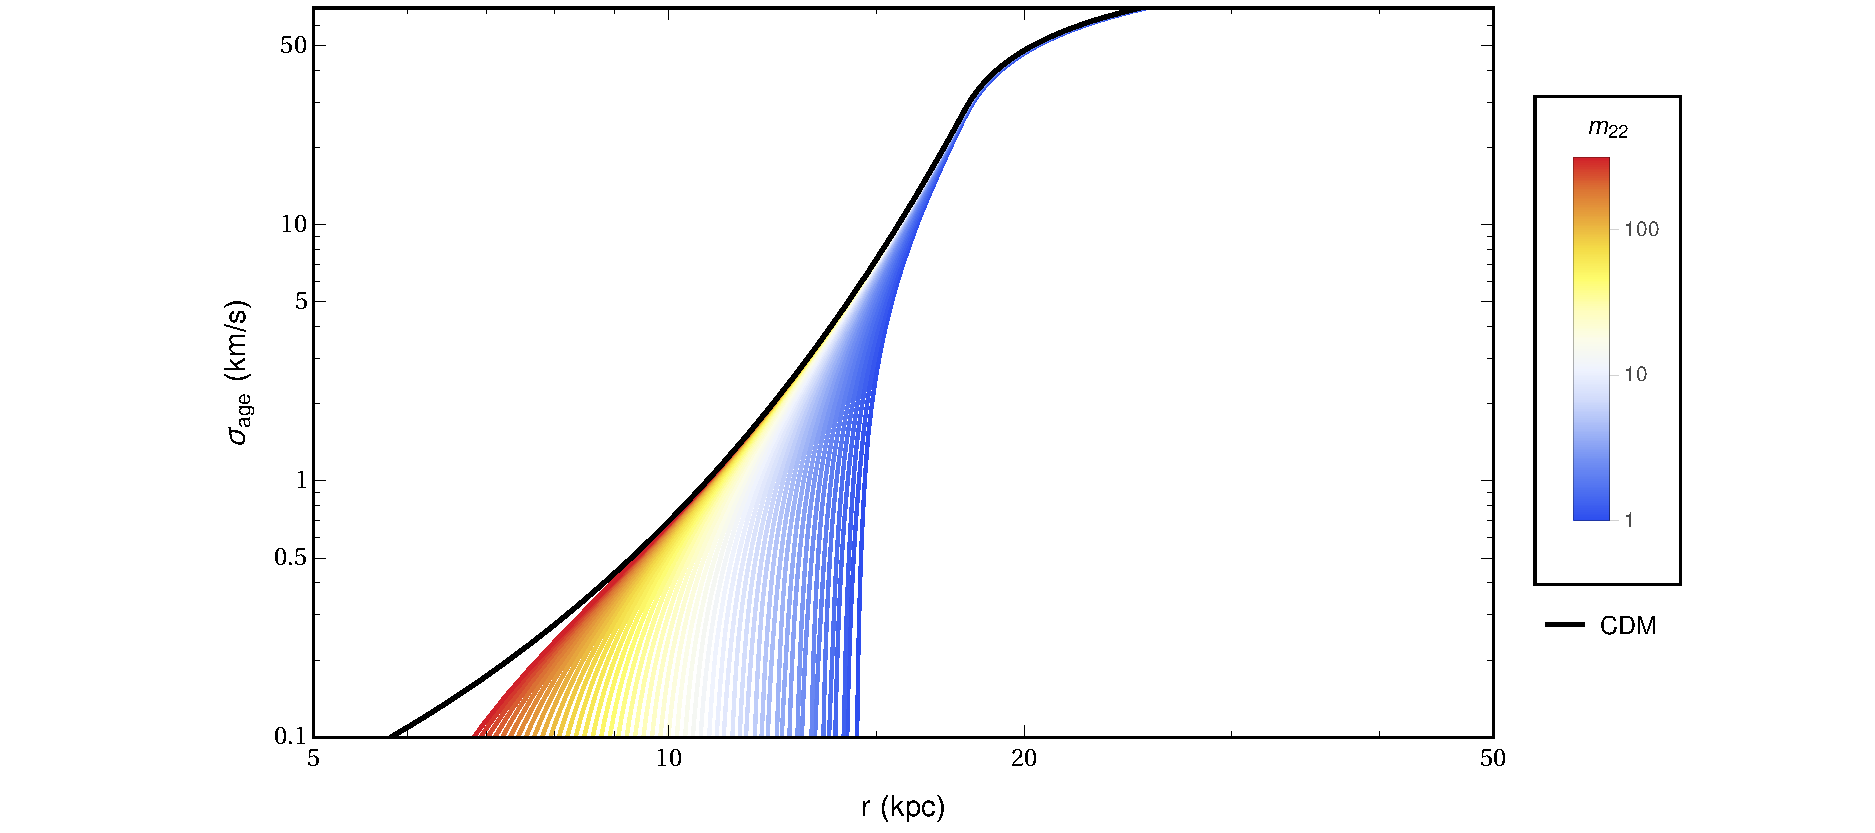
\includegraphics[width= 17cm]{CDM_velocity}
\caption{Rate of heating due to dynamical subhalos as a function of radius for a Milky Way-like halo. The heating is calculated for subhalos in CDM and FDM with a mass range $1 \le m_{22} \le 10^{2.5}$ coloured on a logarithmic scale. Note that FDM subhalos are less effective at small radii due to a deficiency of small FDM subhalos below the quantum scale and the greater effectiveness of tidal disruption.}
\label{fig:CDMheating}
\end{figure*}

\begin{figure*}
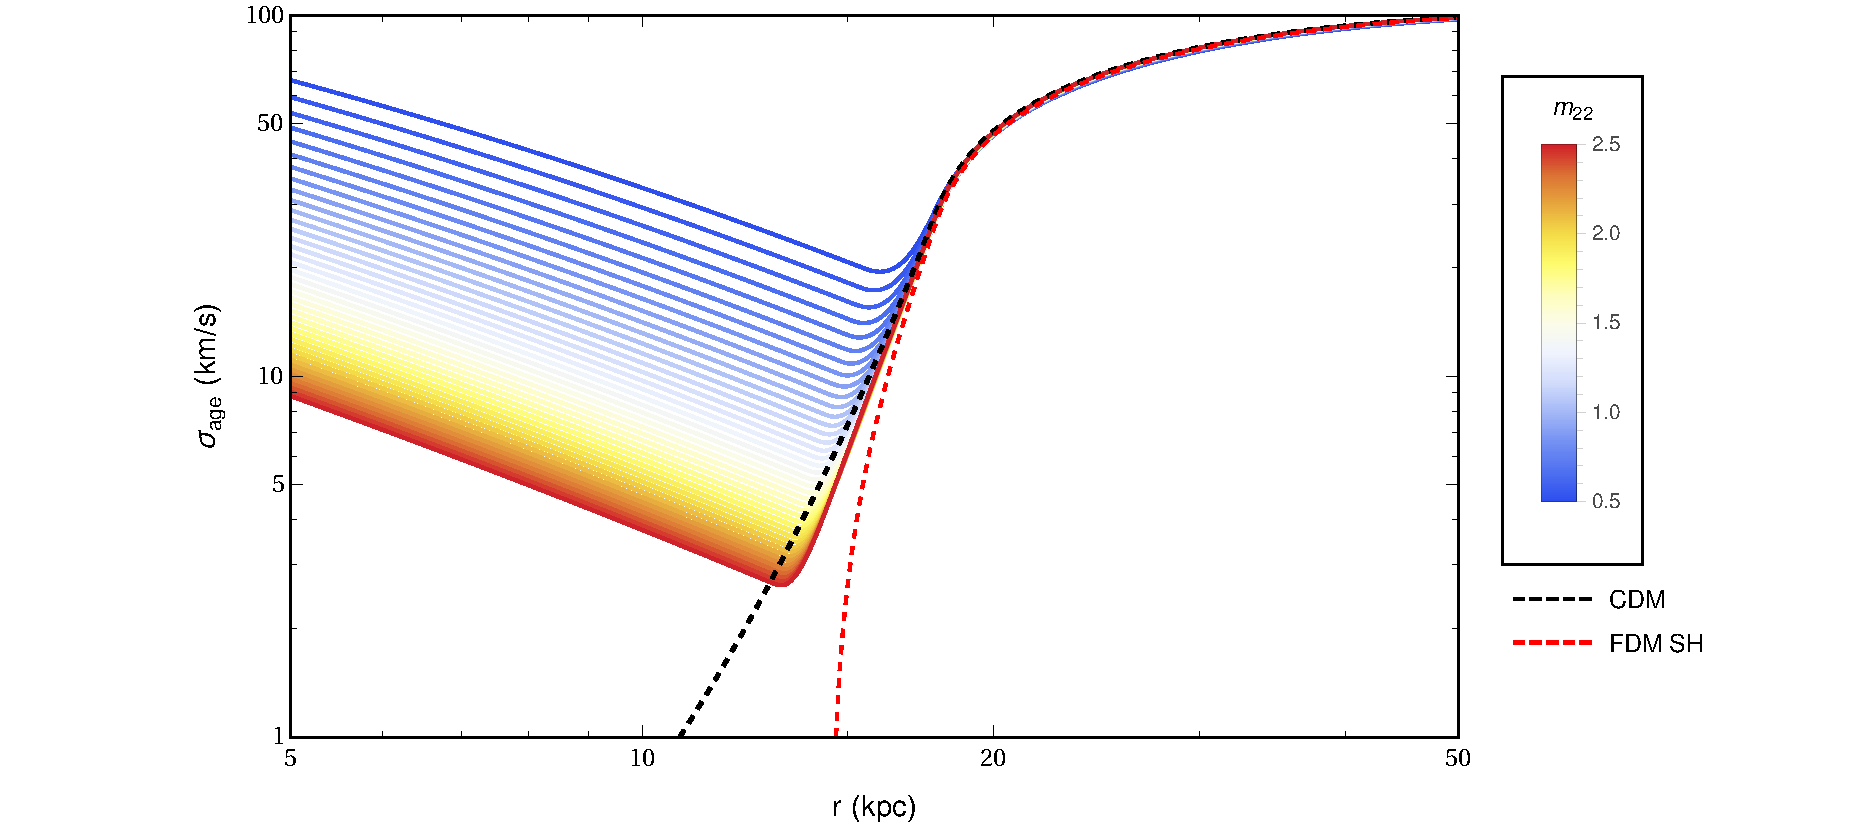
\includegraphics[width=17cm]{FDM_velocity}
\caption{Total Rate of heating due to FDM wavelets and subhalos as a function of radius for axion masses $m_{a}$ in the range \SIrange{0.25 e-22}{ 1.75 e-22}{\electronvolt}. for a Milky Way-like halo. Dashed lines give the heating to subhalos alone in the CDM and FDM models (with $m_{22} = 1$) respectively.}
\label{fig:radiusheating}
\end{figure*}



\subsubsection{The Subhalo Mass Function}

The fluctuations due to subhalos dynamics are reduced in FDM compared to CDM because the halo mass function is suppressed at low mass due to the quantum Jeans scale. The FDM halo mass function is calculated numerically from the Press--Schechter formalism \citep{substructure_FDM, marsh} and the soliton profile is fitted from simulations by \cite{schive_solitons}. 



\subsubsection{Tidal Disruption}

 
We employ an identical method for truncating subhalos due to the tidal stripping of the primary halo. However, in FDM, light subhalos are more easily tidally disrupted via a runaway soliton reformation effect. Since the mass and radius of a soliton are inversely related \citep{solitons}, if the tidal radius of a subhalo lies within its soliton core then mass from the soliton will be stripped away which, due to the self-gravitating quantum condition,
\begin{equation}
R \approx \frac{\hbar^2}{m_a^2 M G},
\end{equation} 
forces the soliton to grow in size causing a runaway effect which completely destroys the subhalo. This runaway process occurs because, as mass is stripped from the soliton, the soliton grows due to quantum pressure (previously halted by gravitational attraction) which pushes more mass outside the tidal radius. To implement this runaway effect, we modify our truncation function by setting $T_R(m) = 0$ if the tidal radius lies within the soliton radius. 

	Furthermore, due to the solitonic cores in FDM, the remaining mass fraction after tidal disruption is strongly dependent on the subhalo mass because the shape of the soliton profile and behavior are strongly mass-dependent. The decline in heating rate due to subhalos within \SI{20}{\kilo\parsec} shown in Figure \ref{fig:CDMheating} is due to tidal destruction. Note that FDM subhalos are less effective at small radii due to a deficiency of small FDM subhalos below the quantum scale and the greater effectiveness of tidal disruption. We can now compare the heating due to subhalos in the FDM and CDM paradigms and a function of the particle mass. The results are summarized in table \ref{table:FDM_ratio}. Note that subhalo-induced heating is vastly suppressed in FDM with a low particle mass due to the combination of enhanced truncation and the suppression of small-scale power below the quantum scale. Because the enhanced truncation is due to a runaway process, the tidal disruption of FDM subhalos is highly sensitive to the tidal radius and therefore the position of the subhalo within the primary halo.
This effect is apparent in the steeper decline,  due to tidal destruction, of the heating rate of subhalos for FDM within \SI{20}{\kilo\parsec} as illustrated in figure \ref{fig:CDMheating}.
 



\subsubsection{Fluctuations due to Wavelets}

Although the fluctuations due to subhalo transits are reduced in the FDM paradigm in comparison to CDM, for a moderately light particle mass ($m_a \approx \SI{e-22}{\electronvolt}$) the dominant effect is due to wavelets, the interference fringes produced by standing FDM waves. In the limit of large particle mass, FDM recreates the results of CDM since the subhalos act identically and the power in wavelets is strongly suppressed by a factor of $m_{22}^{-3}$. For very low particle masses, this power grows rapidly and easily exceeds observational bounds for the velocity dispersion of the Milky Way thick disc. We are primarily interested in the intermediate region in which the transition from wavelet dominated fluctuations to subhalo dominated fluctuations occurs. Figure \ref{fig:radiusheating} illustrates that the transition from wavelet dominated heating to subhalo dominated heating occurs approximately at $r \approx \SI{20}{\kilo \parsec}$. For large particle mass, $m_{22} \approx \SI{2.5e-22}{\electronvolt}$, the minimal heating occurs at $r \approx \SI{10}{\kilo \parsec}$. The radius of the minimal heating increases with decreasing particle mass. Furthermore, as the particle mass decreases, the transition between the wavelet dominated and subhalo dominated regimes becomes smoother and the minimum between the two regimes is ameliorated.   



\begin{figure}
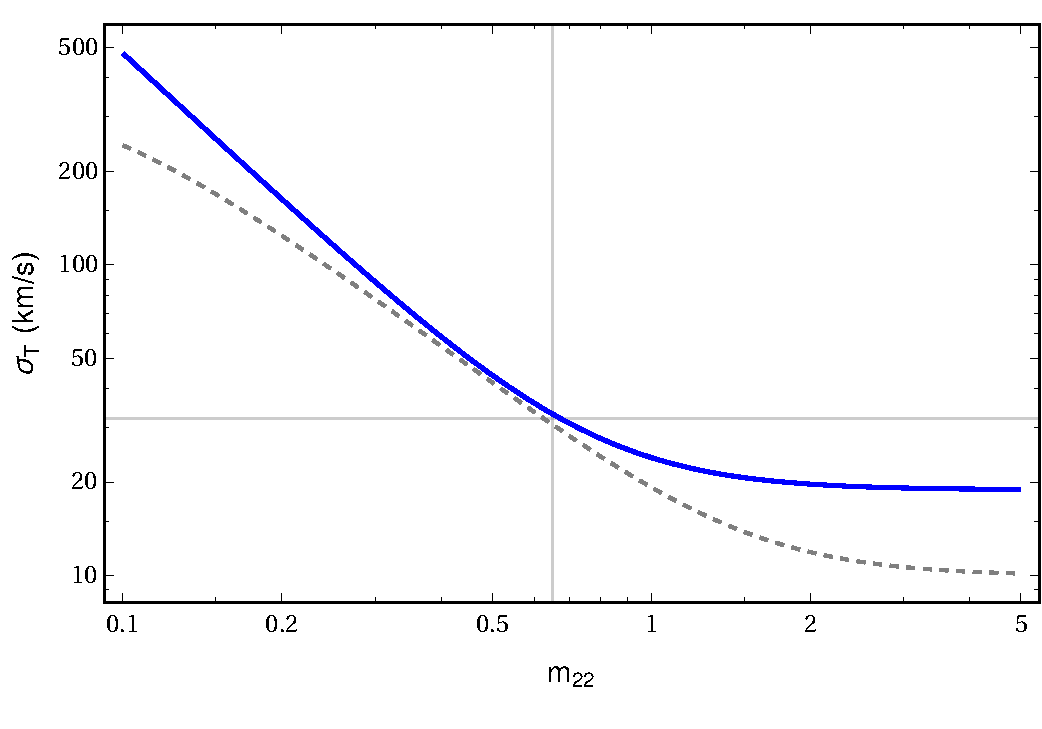
\includegraphics[width=\columnwidth]{FDM_mass_dep}
\vspace*{-5mm}
\caption{Accumulated velocity dispersion at the solar neighborhood $R_{\odot} = \SI{8.3}{\kilo\parsec}$ as a function of axion masses $m_{a}$ in the range \SIrange{0.1 e-22}{ 5 e-22}{\electronvolt} for a Milky Way-like halo. The horizontal line is fixed at $\SI{32}{\kilo\meter\per\second}$, the observational maximum on velocity dispersion of the Milky Way thick disc. The dashed line represents the accumulated velocity dispersion calculated without taking into account the time dependence of the Coulomb logarithm due to increase in oscillation period with disk velocity dispersion.}
\label{fig:mass_dep_heating}
\end{figure}

\begin{table} 
\begin{center}
 \begin{tabular}{||c c||} 
 \hline
 $m_{22}$ & $\left( \frac{\sigma_{FDM}^2}{\sigma_{CDM}^2} \right)^{\tfrac{1}{2}}$ \\ [2.5ex] 
 \hline\hline
 0.75 & 31.88 \\ 
 \hline
 1.00 & 21.39 \\
 \hline
 1.50 & 12.15 \\
 \hline
 2.00 & 8.119 \\
 \hline
 3.00 & 4.587 \\
 \hline
 4.00 & 3.054 \\
 \hline
 5.00 & 2.226 \\
 \hline
 10.00 & 0.830 \\ [1ex] 
 \hline
\end{tabular}
\end{center}
\caption{The ratio of total heating due to FDM substructure and heating due to CDM subhalos at the solar neighborhood $R_{\odot} = \SI{8.3}{\kilo\parsec}$ as a function of particle mass $m = m_{22} \times \SI{e-22}{\electronvolt}$. Here we take the most probable value $A = 2.2$.}
\label{table:FDM_ratio}
\end{table}

\begin{table} \label{FDM_ratio}
\begin{center}
 \begin{tabular}{||c c c||} 
 \hline
 $m_{22}$ & $A^{\tfrac{1}{2}} \left( \frac{\sigma_{SH}^2}{\sigma_{W}^2} \right)^{\tfrac{1}{2}}$ & $ \left( \frac{\sigma_{SH}^2}{\sigma_{W}^2} \right)^{\tfrac{1}{2}} \bigg|_{A = 2.2}$ \\ [2.5ex] 
 \hline\hline
 0.75 & 0.038 & 0.025 \\ 
 \hline
 1.00 & 0.321 &  0.256 \\
 \hline
 1.50 & 1.066 &  0.718 \\
 \hline
 2.00 & 1.957 &  1.319 \\
 \hline
 3.00 & 4.080 & 2.751 \\
 \hline
 4.00 & 6.568 & 4.428 \\
 \hline
 5.00 & 9.362 &  6.312 \\
 \hline
 10.00 & 26.88 & 18.12 \\ [1ex] 
 \hline
\end{tabular}
\end{center}
\caption{The ratio of heating due to FDM subhalos to the heating due to FDM wavelets at $r = \SI{13}{\kilo\parsec}$ as a function of particle mass $m = m_{22} \times \SI{e-22}{\electronvolt}$. The values are quoted both as a function of the amplitude $A$ and for the value $A = 2.2$. }
\end{table}

\section{Discussion}

\begin{figure*}
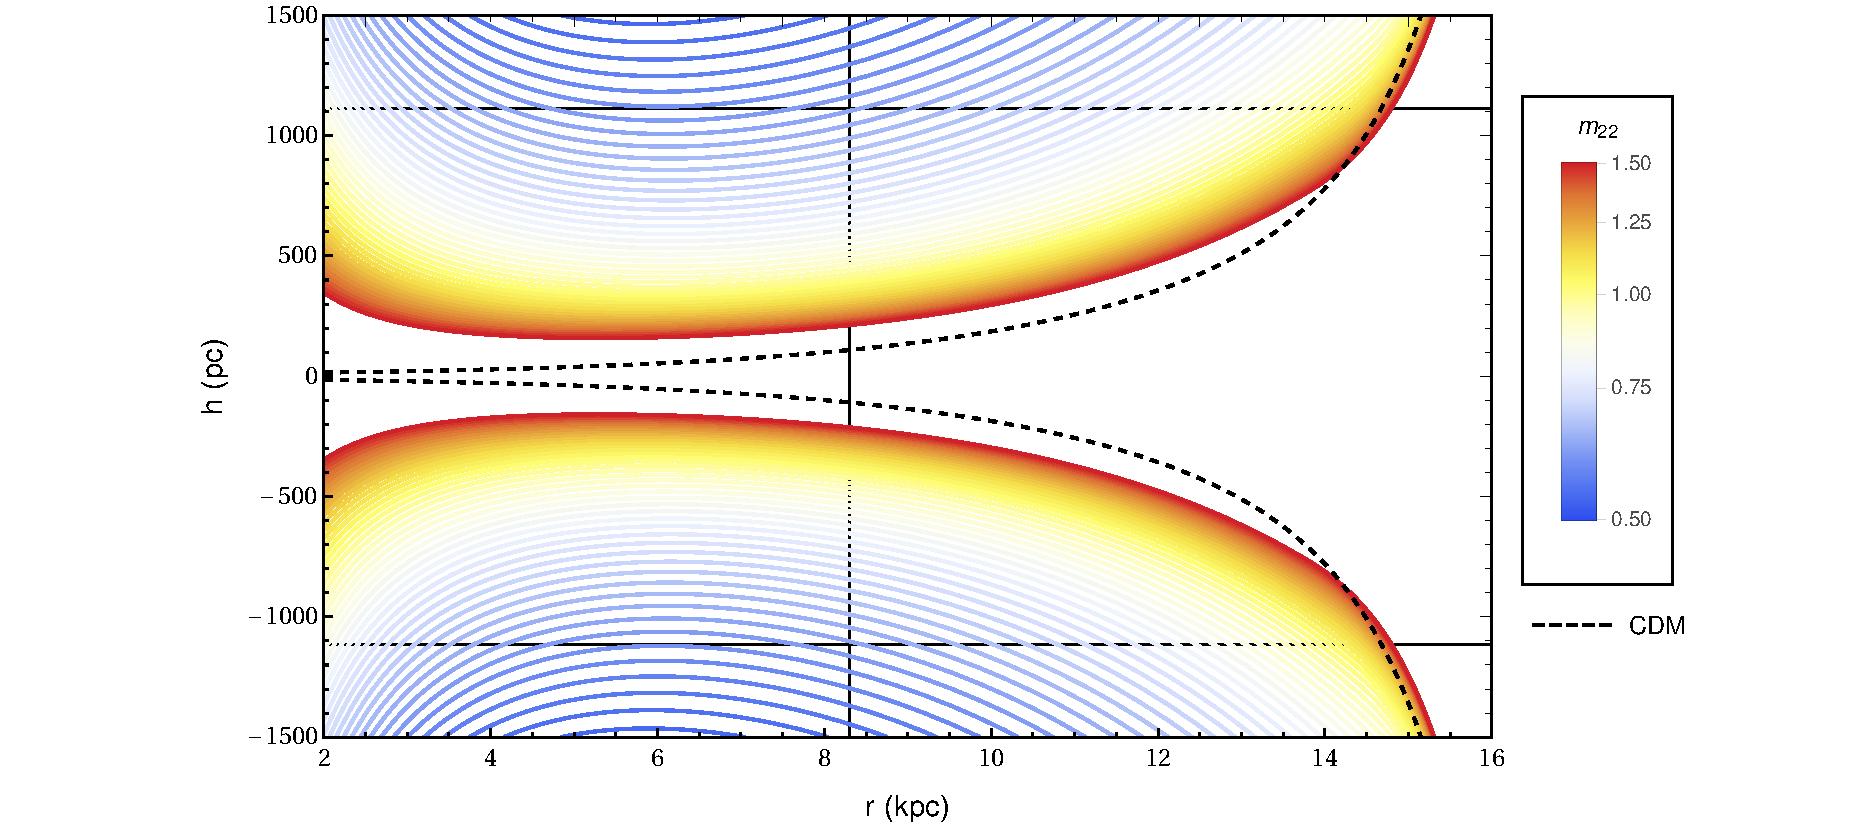
\includegraphics[width=18cm]{disk_shape}
\vspace*{-5mm}
\caption{Profile of the galactic disc thickness induced by substructure heating as a function of radius for a Milky Way-like halo. The vertical velocity dispersion of the disc is assumed to be entirely produced by heating due to FDM wavelets. }
\label{fig:disc_shape_FDM}
\end{figure*}

\begin{figure*}
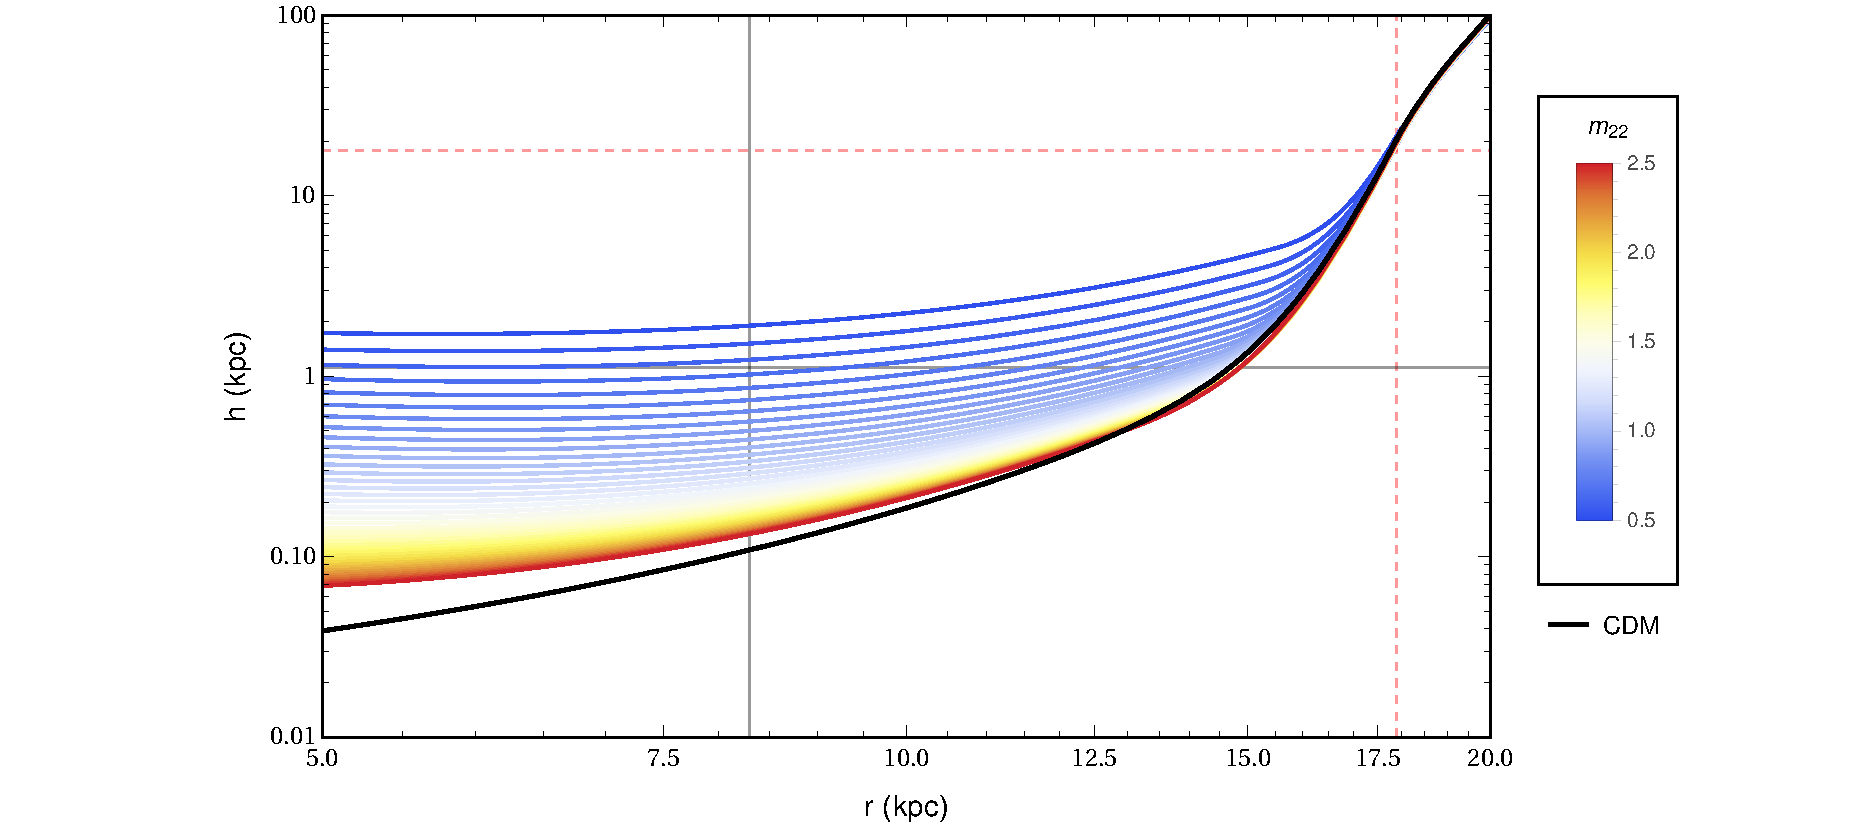
\includegraphics[width=18cm]{disk_scale_height}
\vspace*{-5mm}
\caption{Galactic disc scale height induced by substructure heating as a function of radius for a Milky Way-like halo. The vertical velocity dispersion of the disc is assumed to be entirely produced by heating due to FDM wavelets. The light gray lines mark the point of complete disc destruction. }
\label{fig:disc_scale_height}
\end{figure*}

\subsection{disc Destruction at Large Radii}

Given a dark matter paradigm, we have shown how to estimate the heating of the disc caused by dynamical substructure. If we make the further assumption that dark substructure is the dominant disc thickening effect then we have a method of predicting the actual velocity dispersion of a disc as a function of radius. However, in a galaxy with a known surface density profile, there is a simple relationship between the velocity dispersion and the scale height of a disc given by equation \eqref{scale}. Therefore, we can compare the disc shapes predicted by CDM and FDM shown in figure \ref{fig:disc_shape_FDM} respectively. Subhalos alone cause very little thickening out to a radius of approximately $\SI{15}{\kilo \parsec}$ at which point the disc flares exponentially. This rapid growth in thickness will cause the outer disc to become unstable and lead to disc destruction beyond a certain radius. FDM wavelets produce a more leisurely disc flare beginning near $r \approx \SI{10}{\kilo \parsec}$ before transitioning into the subhalo driven exponential flare at $\SI{15}{\kilo \parsec}$. The wavelet induced gentle flare with a slope of roughly $\beta = 0.1$ (that is $\SI{100}{\parsec}$ of scale height per parsec of radius) is consistent with LAMOST survey data which indicate a strong flaring phenomenon of all stellar populations and, in particular, a flaring slope of $\beta = 0.124$ for the thick disc \citep{LAMOST}. 
\par 
We consider a possible criteria to determine the point at which a galactic disc is destroyed by thickening,
\begin{equation}
\frac{h(r)}{r} > 1.
\end{equation}
This clearly gives an upper bound on the endpoint of the disc. Using this criterion, if the disc is thickened by CDM subhalos alone then the disc will be destroyed past a radius of about $r = \SI{19}{\kilo \parsec}$. Figure \ref{fig:disc_scale_height} shows that the disc shape is not highly sensitive to particle mass at large radii and therefore to the total rate of heating. Therefore, CDM and FDM paradigms do not significantly differ in predicting disc destruction. In fact, the disc flare is mostly determined by density profile of the disc itself.  
\par
FDM wavelets on the other-hand can produce significant thickening at all radii. For example, near the solar neighborhood $r \approx R_{\odot}$, an axion of mass $m_a = \SI{0.5 e-22}{\electronvolt}$ will lead to a scale height of $\SI{469}{\parsec}$ if both disc heating processes are effective. If only the lower bound given by tidal effects is allowed then the time scale over which significant disc thickening occurs is much longer than the current age of the universe \citep{ultralight}. Wavelets will also give rise to exponentially flaring discs. However, because wavelets produce their maximum power at small radii and subhalos at large radii, the disc flaring caused by wavelets is significantly weaker than the CDM counterpart. Furthermore, the transition point from an approximately flat disc to a flaring disc is highly sensitive to particle mass. Therefore, the radius at which disc destruction takes place is quite sensitive to $m_{22}$ although it will be at a larger radii than then comparable CDM number because there are fewer low mass subhalos predicted by FDM than by CDM. 


\subsection{Constraints on Particle Mass}

The Milky Way disc has two components, a recently formed thin disc with low velocity dispersion and a old thick disc with large relatively large velocity dispersion. The thick disc has locally a velocity dispersion of approximately $\SI{32}{\kilo\meter\per\second}$ in its thickest parts \citep{milky_way}. Therefore, the velocity dispersion caused by substructure heating cannot exceed this value. We find that CDM does not produce sufficient heating to be constrained by observational measurements of the local  Milky Way disc. However, the heating due to wavelets in FDM is strongly dependent on particle mass and far more efficient than other substructure. In the low-mass limit, the heating may vastly exceed observational bounds. Using the results quoted for the velocity dispersion of the thick disc as a strict cutoff, we derive a lower bound on the mass of the FDM particle,
\begin{equation}
m_a > 0.43 A^{1/3} \times \SI{e-22}{\electronvolt}
\end{equation}
Using the numerical estimate, $A \approx 2.2$, we obtain the most probable lower bound at $2 \sigma$ confidence on the FDM particle mass of,
\[ m_a > 0.57 \times \SI{e-22}{\electronvolt} \]
under the assumption that all disc heating is reflected in the z-velocity dispersion. If we further assume that dynamical FDM substructure is the primary source of disk heating then the vertical velocity dispersion in the solar neighborhood constrains the entire heating profile at all radii. For the most probable value of $m_{22}$ the maximum heating occurs at $r = \SI{1.3}{\kilo \parsec}$ with a value of $\sigma_{10} = \SI{81}{\kilo\meter\per\second}$. The entire heating profile for this value of the FDM particle mass is shown in figure \ref{fig:heating_shape}. We hope that detailed studies to the Milky Way disk stars outside the solar neighborhood made possible by recent Gaia data will test the validity of this proposed heating curve.   

\begin{figure}
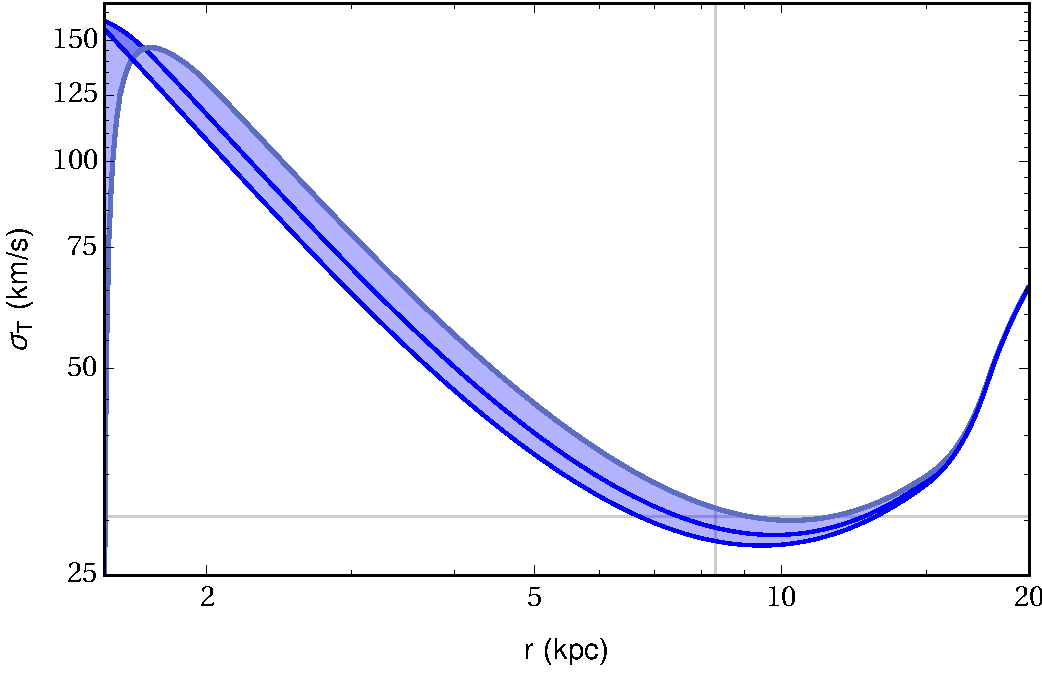
\includegraphics[width=\columnwidth]{heating_shape}
\vspace*{-5mm}
\caption{Heating profile as a function of radius for the most probable value of $m_{a} = \SI{0.59 e-22}{\electronvolt}$ under the assumption that FDM substructure is the primary mode of disk heating. Error bars are given at the $1 \sigma$ level. }
\label{fig:heating_shape}
\end{figure}

\subsection{Heating History}

A source of contention between our theoretical treatment and observation is our prediction for the heating history of the disc. Both dark matter paradigms predict a constant rate of heating independent of the velocity dispersion of the disc and therefore a time dependent velocity dispersion $\sigma_D \approx t^{\beta}$ with $\beta = \tfrac{1}{2}$. This disagrees with analyses which suggest that the Milky Way thick disc has increased in velocity dispersion with exponent $\beta \approx \tfrac{1}{3}$ \citep{heating_history}. However, these calculations assume that dark substructure alone (ignoring, for example, the contribution due to spiral structure heating effective at low values of $\sigma$) is responsible for disc heating. Multiple sources of heating may combine to produce a lower effective exponent. However, the above results are possibly disputed by the recent findings of \cite{Gaia_vertical_motions} drawing upon APOGEE and Gaia data to estimate vertical heating as a function of age. In the solar neighborhood, they find that the vertical action scales with age as $\widehat{J}_z \propto t^{\gamma}$ for $\gamma \approx 1$ which is approximately a heating history of $\sigma \propto t^\beta$ with $\beta \approx \frac{1}{2}$. Superficially, this is inconsistent with heating due primarily to GMC scattering which predicts $\beta = \frac{1}{4}$. However, $\widehat{J}_z$ is not exactly the evolutionary heating path but reflects both the action of starts at birth and their subsequent heating history. \cite{Gaia_vertical_motions} argue GMC scattering can be salvaged to be consistent with $\gamma \approx 1$ if the scattering amplitudes and heating efficacy are functions of time in a certain physically reasonable way. However, heating due to dynamical substructure automatically predicts a heating history of the thin disc consistent with the observed value $\gamma \approx 1$ without the need for time-dependent parameters as well as explaining the existence of the thick disc which GMC scattering does not. In fact, the heating we predict from FDM substructure naturally explains the phenomenon of increasing vertical action with radius in the range 10-\SI{15}{\kilo \parsec}. 
That said, our analysis fails to explain the gradual observed increase in $\gamma$ as a function of radius and predicts a greater degree of heating to the interior of the disc within $R_{\odot}$ than is found by \cite{Gaia_vertical_motions}. If both FDM substructure and GMC scattering operate in line with the current understanding, it is plausible, if not likely, that a combination of these effects best explains the heating data. 

\subsection{Conclusion and Comparisons With Other Current Work}

We find that the heating of Milky Way type stellar discs by substructure gravitational fluctuations will lead to flaring and disc destruction at radii greater than \SIrange{15}{20}{\kilo\parsec} in both CDM and FDM paradigms. However, quantum wavelets in FDM can be effective at heating the inner disc regions accounting for the thick disc and the observed flaring of star populations. A particle mass in excess of $m_a > \SI{0.57 e-22}{\electronvolt}$ is required to avoid exceeding observational bounds on heating of thick disc stars in the Milky Way. Correspondingly, an FDM scenario with particle mass $m_a \approx \SI{e-22}{\electronvolt}$ can, in fact, explain the observed increase in velocity dispersion with increasing stellar age observed in the solar neighborhood.  
\par
The contemporary study by \cite{stellar_streams_bound} has also determined a lower bound on the mass of the FDM axion using similar methodology to study the thickening of thin stellar streams by FDM wavelets. These calculations exhibit the same scaling in terms of $m_{22}$ and similar heating versus time profiles. Thin stellar streams give a stricter lower bound of $m_a > \SI{1.5 e-22}{\electronvolt}$ than our analysis of disc thickness. While an axion mass in excess of $\SI{1.5 e-22}{\electronvolt}$ is insufficient to explain the thick disc alone, it is worth noting that galactic processes from multiple regimes suggest FDM models with particle masses within small numerical factors.    
\par 
\cite{relaxation} recently considered relaxation processes in the FDM paradigm by studying diffusion in stochastic density fields. Of many results, the authors calculate an effective heating timescale for FDM fluctuations to pump energy into massive bodies of
\begin{equation}
T_{\text{heat}} = \frac{3 m_a^3 \sigma^6}{16 \pi^2 G^2 \rho^2 \hbar^2 \log{\Lambda_{\text{FDM}}}} .
\end{equation}  
This effective heating timescale exhibits the same scaling relations and is comparable to the ratio we, from our own analysis, find between the heating rate and the velocity dispersion of the halo. Explicitly,
\begin{equation}
\left( \frac{1}{\sigma_H^2} \deriv{\sigma_D^2}{t} \right)^{-1} = \frac{3 \sqrt{3} m_a^3 \sigma_H^6}{16 \pi^4 A G^2 \rho^2 \hbar^2 \log{\Lambda_{\text{FDM}}}} = \frac{\sqrt{3} }{A \pi^2} T_{\text{heat}}.
\end{equation}
Furthermore, \cite{relaxation} explicitly calculate the effective timescale for the heating of a spherical population of stars in equation (103). The authors find that, for a singular isothermal spherical halo with parameters comparable to the halo of the Milky Way, FDM heating is only significant at radii less than $\sim \SI{1}{\kilo \parsec}$. This, however, does not contradict the results discussed in this paper, primarily because $T_{\text{heat}}$ gives the timescale over which FDM fluctuations pump enough energy into massive bodies for their velocity dispersion to become comparable to the velocity dispersion \textit{of the FDM halo}. This far exceeds the required heating to account for the thickening of a galactic disc because the vertical velocity dispersion of the disc is about an order of magnitude smaller than that of the halo. Furthermore, the singular isothermal sphere is not a good model for density profile of an FDM halo near the solar radius. Since $R_{\odot}$ is within the core radius of the primary halo for reasonable estimates of the NFW halo of the Milky Way, we expect that the density profile goes as $r^{-1}$ rather than $r^{-2}$ as predicted by the singular isothermal sphere model. Essentially, this discrepancy is due to the fact that, near the solar neighborhood, the mass of the Milky Way disc accounts for a significant fraction of the orbital velocity and thus the halo alone does not produce a flat rotation curve (which would imply a singular isothermal sphere). Therefore, the density, the size of FDM density fluctuations, and thus the rate of heating is a less extreme function of radius in a NFW halo than is the model presented by \cite{relaxation}. Near the solar neighborhood, we would expect the actual heating timescale to depend on $r^2$ rather than $r^4$ (c.f. equation (103), \cite{relaxation}). These considerations lead to a modified formula for the heating radius,
\begin{multline}
r_{\text{heat}} = \SI{9.28}{\kilo\parsec} \left( \log{\Lambda} \frac{T_{\text{age}}}{\SI{10}{\giga\year}} \right)^{1/2} \left( \frac{v_c}{\SI{200}{\kilo\meter\per\second}} \right)^{-1} 
\\
 \cdot \left( \frac{m_a}{\SI{0.5 e-22}{\electronvolt}} \right)^{-3/2},
\end{multline}
which is the radius such that heating is effective whenever $r_{\star} < r_{\text{heat}}$. Therefore, heating can be effective near the solar neighborhood when $m_{22} \sim 0.5$. Taking into account the shorter timescale needed to heat the disc up to its current thickness and the less extreme radial falloff in the strength of this heating, the results of \cite{relaxation} are, in fact, consistent with the possibility that FDM fluctuations with a particle mass $m_a = \SI{0.59e-22}{\electronvolt}$ are the cause of the observed thick disc near the solar radius.
\par
It is natural to consider how FDM and CDM substructure may influence the discs of galaxies besides the Milky Way. In general, this is a very difficult because accurate measurements of the halos, discs, and vertical velocity dispersion of other galaxies are quite difficult to obtain. Since our model of dynamical substructure will produce vertical heating to any disc embedded in a dark matter halo, the family of superthin galaxies are a particularly interesting test case. The recent study of the superthin galaxy FGC1540 by \cite{superthin} estimates properties of the galaxy's dark matter halo in enough detail to determine whether the thickness (or lack there of) of FGC1540 is inconsistent with our model.  
Without presenting the details, we can say that the system in question has a very young very thin disc and an older thick disc, with the latter not inconsistent with FDM for particle masses on the order of $\SI{e-22}{\electronvolt}$ and with the constraint derived from the Milky Way thick disc. The thin disc of FGC1540, on the other hand, must be very young, $\sim \SI{2}{\giga \year}$, for FDM heating to be consistent with the observed thickness for $m_{a} \approx \SI{1 e-22}{\electronvolt}$.   

\section*{Acknowledgments}
We thank Mihir Kulakarni for his code to calculate the FDM halo mass function and his invaluable guidance on this project. We further thank Professor Hsi-Yu Schive for helpful discussions on the nature of FDM solitons and wavelets and Professor James Binney for critique and thoughts on the nature and origin of the old disc. Many thanks to Professor Scott Tremaine for his helpful criticism and insights regarding the transfer of energy to disc thickening from bending modes of the disc versus tidal strain. Support (PM) for this work was provided by NASA through the Einstein Postdoctoral Fellowship grant no. PF7-180164 awarded by the Chandra X-ray Center which is operated by the Smithsonian Astrophysical Observatory for NASA under contract NAS8-03060. 


\bibliography{mybib}


 
\end{document}
